%% LaTeX-Beamer template for KIT design
%% by Erik Burger, Christian Hammer
%% title picture by Klaus Krogmann
%%
%% version 2.1
%%
%% mostly compatible to KIT corporate design v2.0
%% http://intranet.kit.edu/gestaltungsrichtlinien.php
%%
%% Problems, bugs and comments to
%% burger@kit.edu

\documentclass[18pt]{beamer}

%% SLIDE FORMAT

% use 'beamerthemekit' for standard 4:3 ratio
% for widescreen slides (16:9), use 'beamerthemekitwide'

\usepackage{templates/beamerthemekit}
% \usepackage{templates/beamerthemekitwide}

%% TITLE PICTURE

% if a custom picture is to be used on the title page, copy it into the 'logos'
% directory, in the line below, replace 'mypicture' with the 
% filename (without extension) and uncomment the following line
% (picture proportions: 63 : 20 for standard, 169 : 40 for wide
% *.eps format if you use latex+dvips+ps2pdf, 
% *.jpg/*.png/*.pdf if you use pdflatex)

\titleimage{treppe}

%% TITLE LOGO

% for a custom logo on the front page, copy your file into the 'logos'
% directory, insert the filename in the line below and uncomment it

\titlelogo{cvhci}

% (*.eps format if you use latex+dvips+ps2pdf,
% *.jpg/*.png/*.pdf if you use pdflatex)

%% TikZ INTEGRATION

% use these packages for PCM symbols and UML classes
% \usepackage{templates/tikzkit}
% \usepackage{templates/tikzuml}

\usepackage[utf8]{inputenc}

% for xml listing
\usepackage{listings}

\usepackage{color}
\definecolor{gray}{rgb}{0.4,0.4,0.4}
\definecolor{darkblue}{rgb}{0.0,0.0,0.6}
\definecolor{cyan}{rgb}{0.0,0.6,0.6}

\lstset{
  basicstyle=\ttfamily,
  columns=fullflexible,
  showstringspaces=false,
  commentstyle=\color{gray}\upshape
}

\lstdefinelanguage{XML}
{
  morestring=[b]",
  morestring=[s]{>}{<},
  morecomment=[s]{<?}{?>},
  stringstyle=\color{black},
  identifierstyle=\color{darkblue},
  keywordstyle=\color{cyan},
  morekeywords={xmlns,version,type}% list your attributes here
}

\lstdefinestyle{xmlListingStyle}{
  language=XML,
  numbers=left,
  stepnumber=0,
  numbersep=10pt,
  tabsize=4,
  showspaces=false,
  showstringspaces=false
}

% for plotting
\usepackage{pgfplots}
\usepackage{mathtools}

% the presentation starts here

\title[Daten/Bilder]{Treppen Detektierung - Daten/Bilder}
\subtitle{Practical Course Computer Vision for Human-Computer Interactionn}
\author{Yang Zhang, Chris Konop, Jasper Zimmer}

\institute{Computer Vision for Human-Computer Interaction Lab}

% Bibliography

\usepackage[citestyle=authoryear,bibstyle=numeric,hyperref,backend=biber]{biblatex}
\addbibresource{templates/example.bib}
\bibhang1em

\begin{document}

% change the following line to "ngerman" for German style date and logos
%\selectlanguage{english}
\selectlanguage{ngerman}

%title page
\begin{frame}
\titlepage
\end{frame}

%table of contents
\begin{frame}{Outline/Gliederung}
\tableofcontents
\end{frame}

\section{Labeling}
\subsection{LabelMe - Annotationstool}
\begin{frame}{LabelMe - Übersicht}
\begin{itemize}
\item Online Annotationstool
\item Web Frontend
\item Vorgabe von Labels, z.B. Stairs
\item Annotation durch Polygone
\end{itemize}
\end{frame}

\begin{frame}{LabelMe - Frontend}
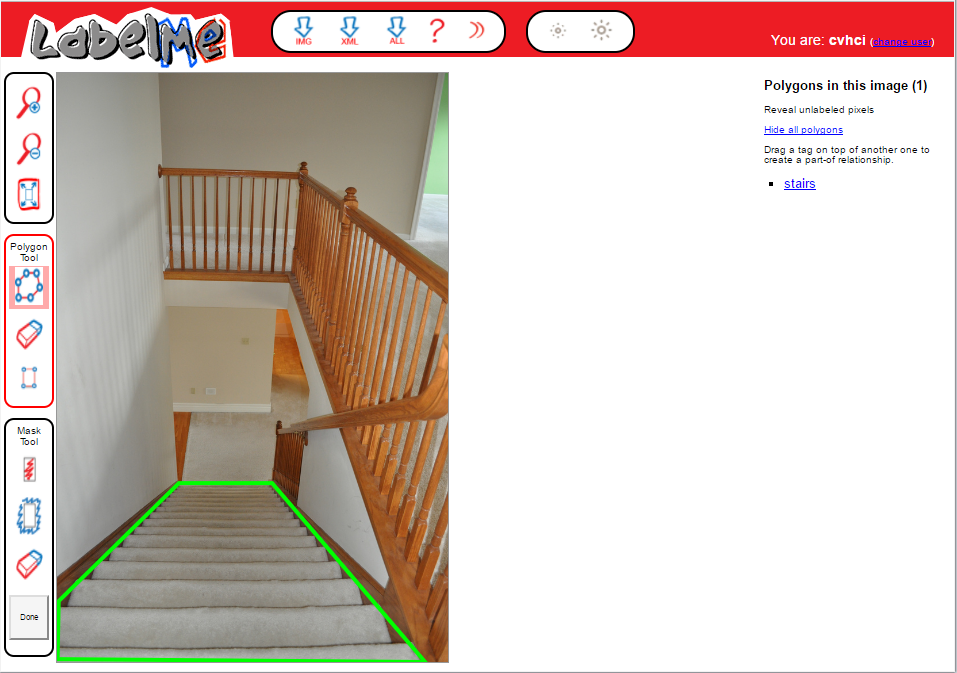
\includegraphics[width=1.0\textwidth, height=0.8\textheight, clip]{images/labelme_example.PNG}
\end{frame}

\begin{frame}{LabelMe - Polygon}
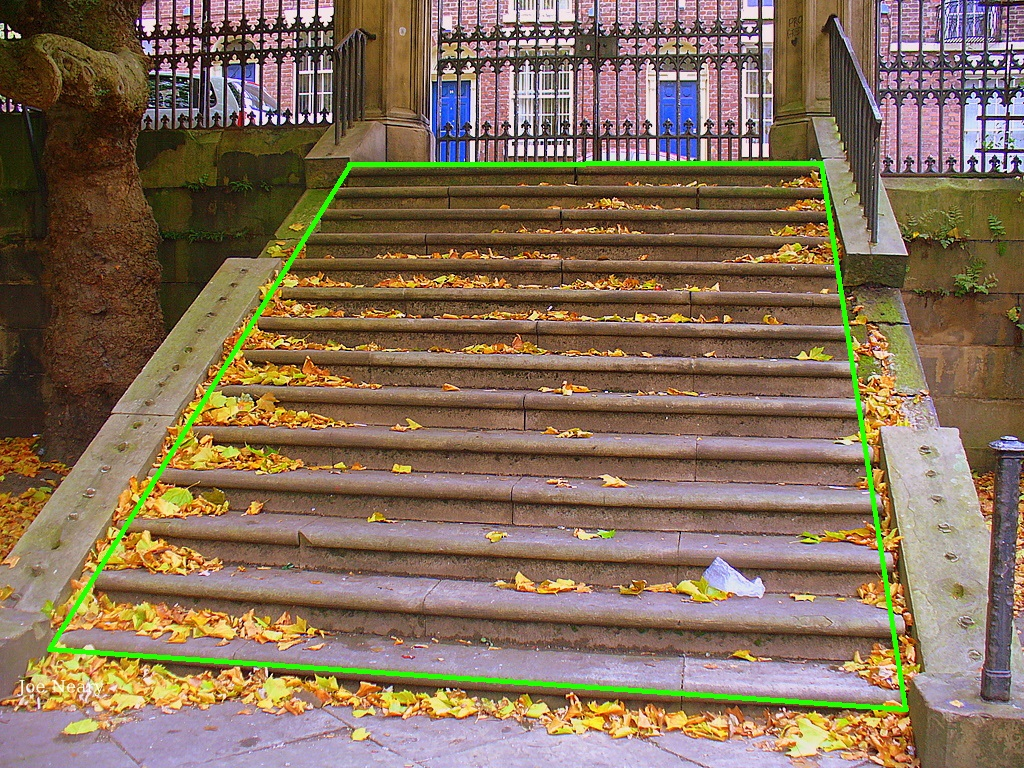
\includegraphics[width=1.0\textwidth, height=0.8\textheight, clip]{labelme_annotated_image/image.jpg}
\end{frame}

\begin{frame}{LabelMe - Annotationen(XML)}
\lstinputlisting[language=XML, firstline=20, lastline=38, basicstyle=\fontsize{10}{10}\selectfont\ttfamily, style=xmlListingStyle]{labelme_annotated_image/annotation.xml}
\end{frame}

\section{Daten}
\subsection{Flickr}
\begin{frame}{Flickr}
\begin{itemize}
	\item Suchbegriffe: \textbf{Treppe, Rolltreppe, Steps, Stairs, Staircase, Escalator}
	\item Bilder insgesamt: \textbf{23949}
	\begin{itemize}
		\item davon nur \textbf{58} Duplikate(Hash)
		\item davon ca. \textbf{30\%} unbrauchbar
	\end{itemize}
	\item Bisher \textbf{3013} Bilder gelabelt
\end{itemize}
\end{frame}

\subsection{Beispiele}
\begin{frame}{Beispiele}
\begin{minipage}[c]{0.4\textwidth}
	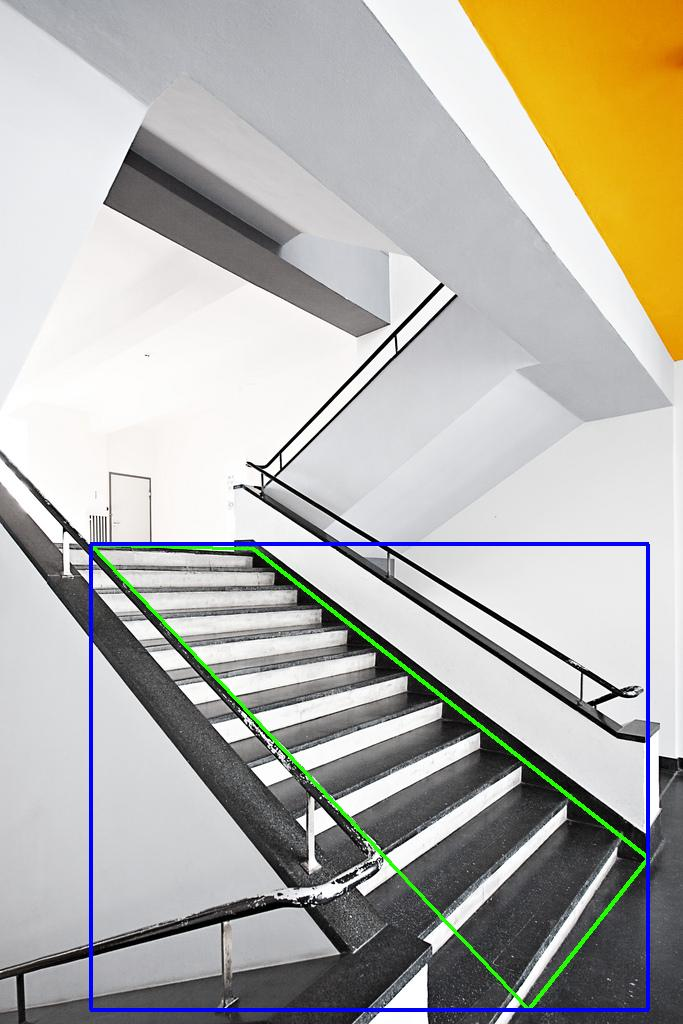
\includegraphics[height=0.8\textheight, clip]{images/flickr_examples/4024886181_f1a802df84_b.jpg}
\end{minipage}
\begin{minipage}[c]{0.18\textwidth}
	\hfill
\end{minipage}
\begin{minipage}[c]{0.4\textwidth}
	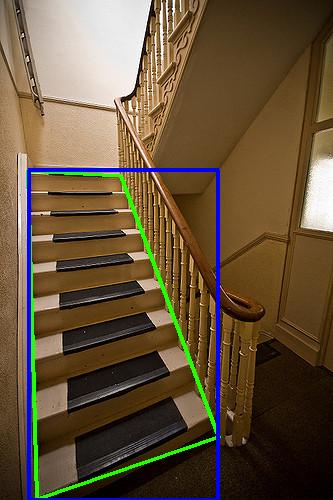
\includegraphics[height=0.8\textheight, clip]{images/flickr_examples/4035000178_2030f90269_z.jpg}
\end{minipage}
\end{frame}

\begin{frame}{Beispiele}
\begin{minipage}[c]{0.4\textwidth}
	\begin{minipage}[c]{0.4\textwidth}
		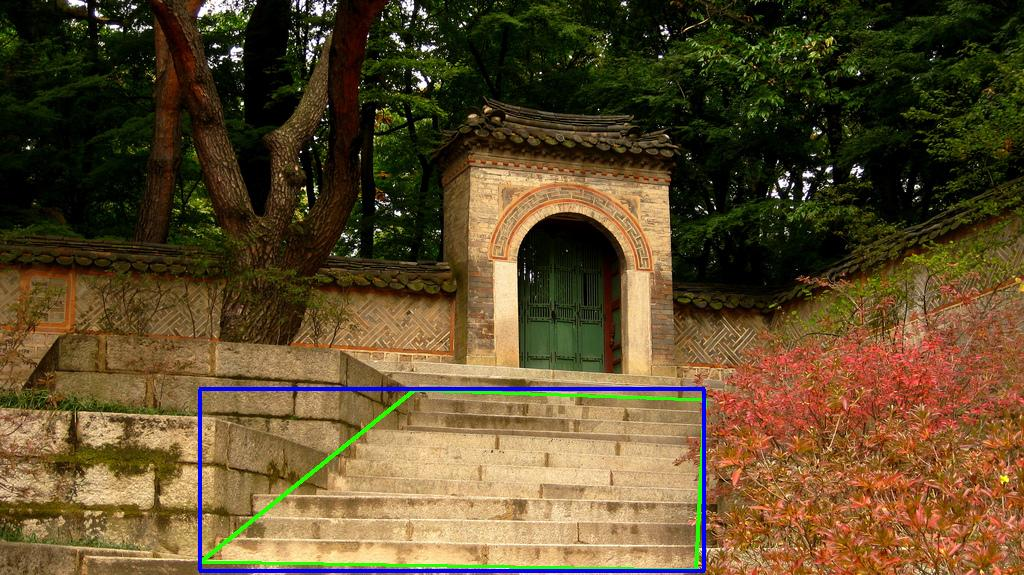
\includegraphics[height=0.35\textheight, clip]{images/flickr_examples/4036295517_82db571311_b.jpg}
	\end{minipage}\\
	\begin{minipage}[c]{0.18\textwidth}
		\vfill
	\end{minipage}\\
	\begin{minipage}[c]{0.4\textwidth}
		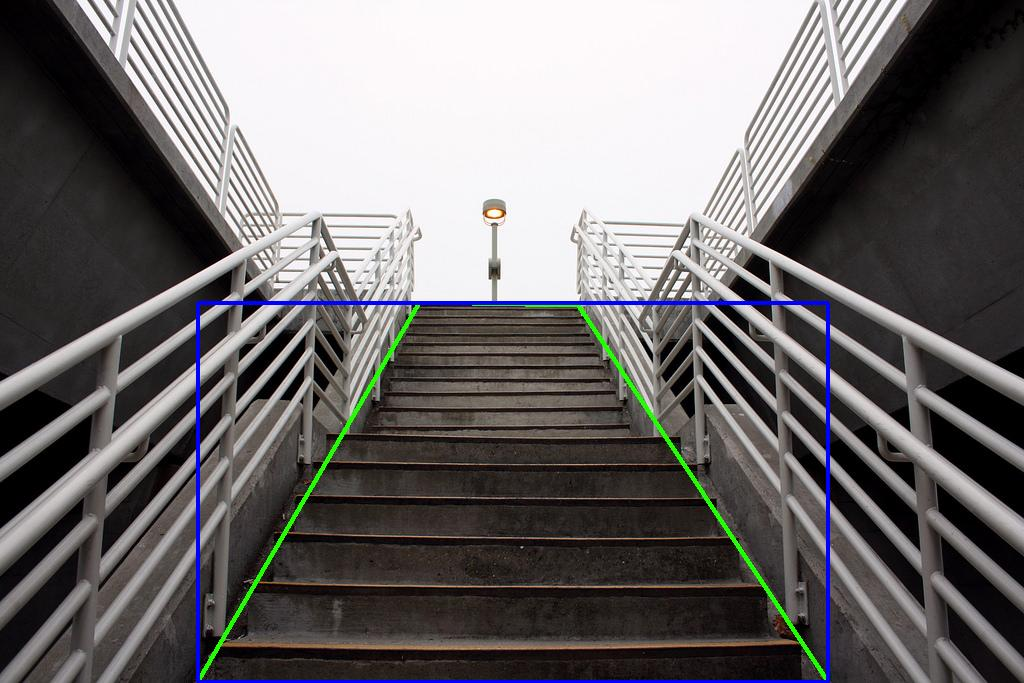
\includegraphics[height=0.415\textheight, clip]{images/flickr_examples/4088220467_3926f18bf8_b.jpg}
	\end{minipage}
\end{minipage}
\begin{minipage}[c]{0.14\textwidth}
	\hfill
\end{minipage}	
\begin{minipage}[c]{0.4\textwidth}
	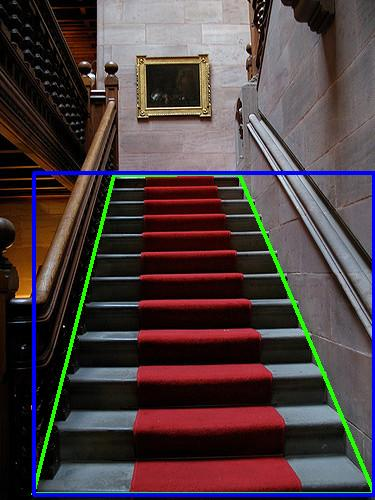
\includegraphics[height=0.8\textheight, clip]{images/flickr_examples/4059454958_cd3d794049_z.jpg}
\end{minipage}
\end{frame}

\begin{frame}{Beispiele}
\begin{minipage}[c]{0.4\textwidth}
	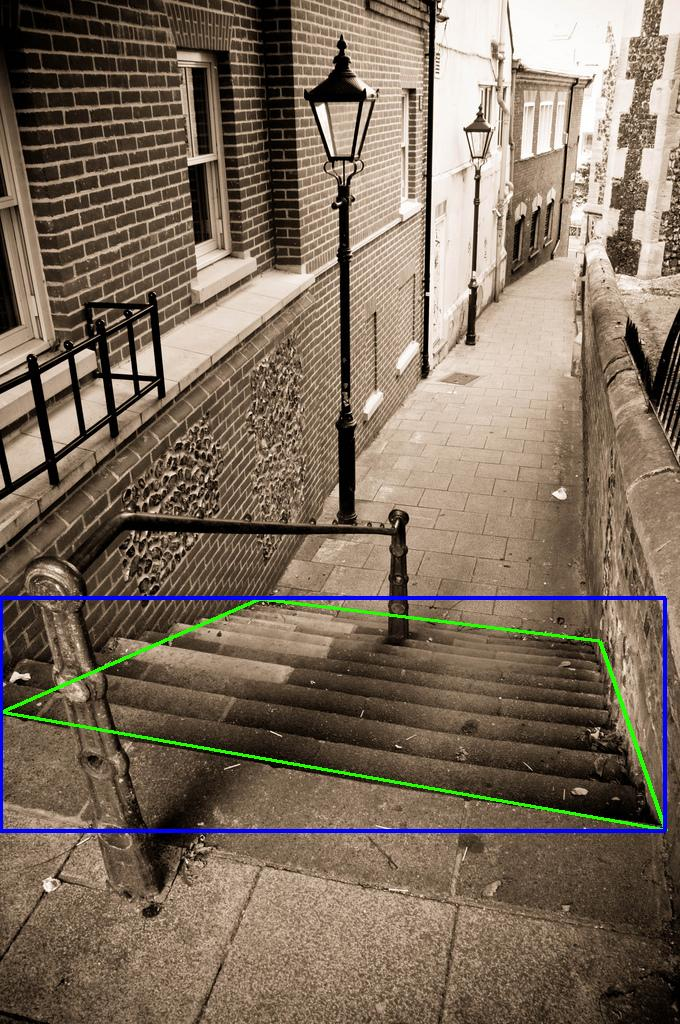
\includegraphics[height=0.8\textheight, clip]{images/flickr_examples/4061458562_295032a441_b.jpg}
\end{minipage}
\begin{minipage}[c]{0.14\textwidth}
	\hfill
\end{minipage}	
\begin{minipage}[c]{0.4\textwidth}
	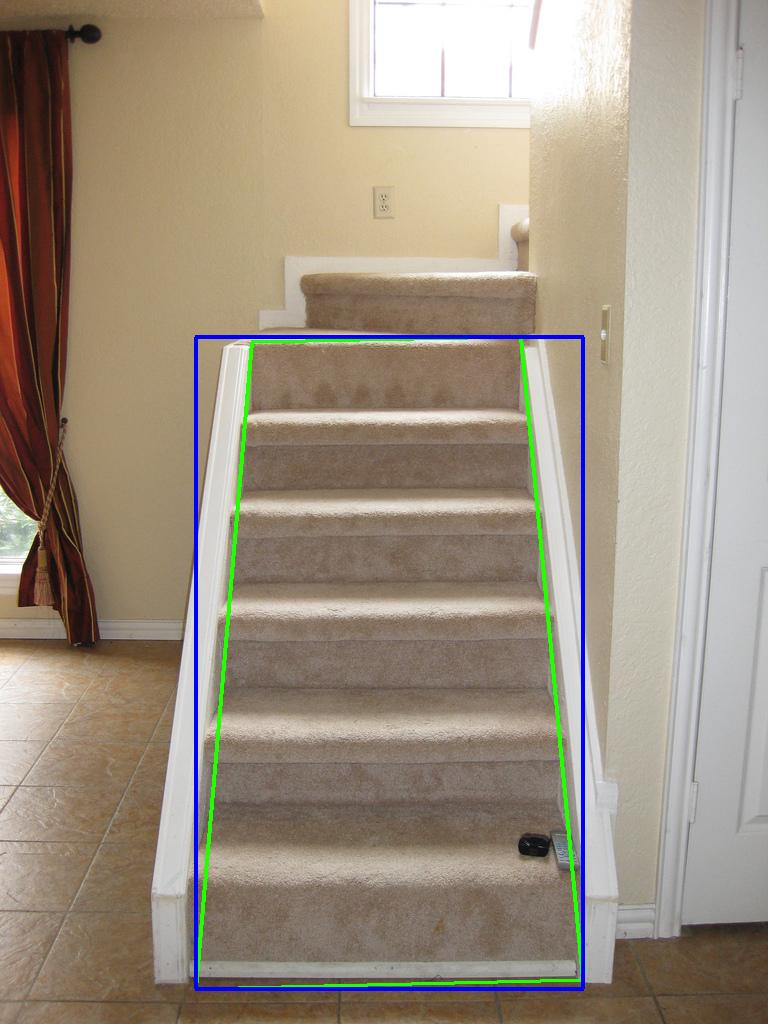
\includegraphics[height=0.8\textheight, clip]{images/flickr_examples/4070233118_fbd77f3112_b.jpg}
\end{minipage}
\end{frame}

\begin{frame}{Beispiele}
\begin{minipage}[c]{0.4\textwidth}
	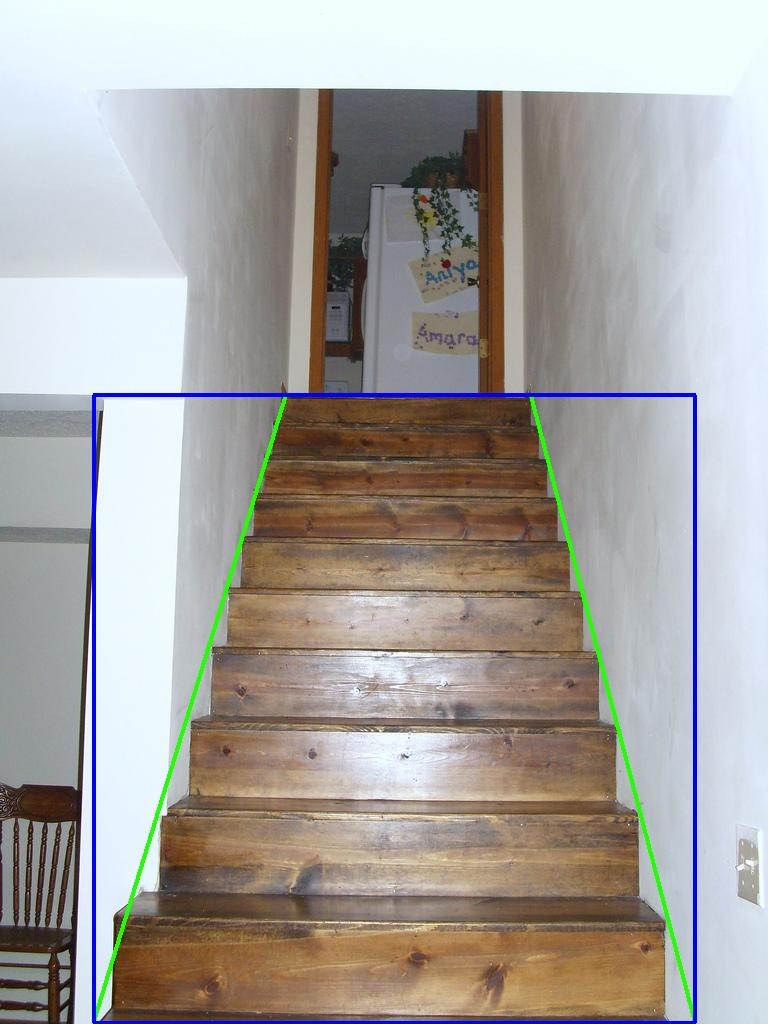
\includegraphics[height=0.8\textheight, clip]{images/flickr_examples/4189244864_6cd6a94b7a_b.jpg}
\end{minipage}
\begin{minipage}[c]{0.18\textwidth}
	\hfill
\end{minipage}
\begin{minipage}[c]{0.4\textwidth}
	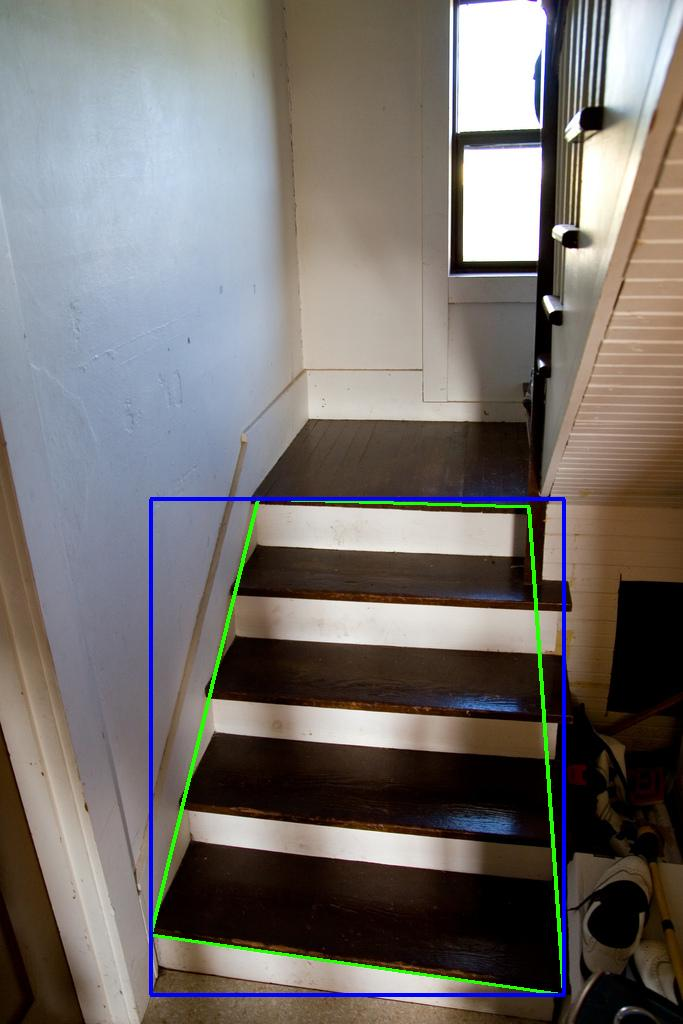
\includegraphics[height=0.8\textheight, clip]{images/flickr_examples/4094167619_9758970368_b.jpg}
\end{minipage}
\end{frame}

\subsection{Verhältnis BoundingBox vs. Bild Größe}
\begin{frame}{Verhältnis - BoundingBox vs. Bild Größe}
\begin{figure}
	\begin{tikzpicture}
	\begin{axis}[width=1.0\textwidth,height=0.8\textheight,
		xlabel={Überdeckung in \%},
		ylabel={Anzahl der Bilder},
		legend pos=north west]
		
		\addplot table[x=Ueberdeckung, y=Anzahl, col sep=comma] {data/box_image_size_ratio.csv};
	\end{axis}
	\end{tikzpicture}
\end{figure}
\end{frame}

\subsection{Verhältnis Polygon vs. BoundingBox Größe}
\begin{frame}{Verhältnis - Polygon vs. BoundingBox Größe}
\begin{figure}
	\begin{tikzpicture}
	\begin{axis}[width=1.0\textwidth,height=0.8\textheight,
	xlabel={Überdeckung in \%},
	ylabel={Anzahl der Bilder},
	legend pos=north west]
	
	\addplot table[x=Ueberdeckung, y=Anzahl, col sep=comma] {data/polygon_box_size_ratio.csv};
	\end{axis}
	\end{tikzpicture}
\end{figure}
\end{frame}

\appendix
\beginbackup

\begin{frame}[allowframebreaks]{References}
\printbibliography
\end{frame}

\backupend

\end{document}
